% Functional specification for ProfiSnort
\documentclass[listof=totoc,a4paper]{scrreprt}

\usepackage[german]{babel}
\usepackage[utf8]{inputenc}
\usepackage[T1]{fontenc}
\usepackage{ae}
\usepackage[bookmarks,bookmarksnumbered]{hyperref}
\usepackage{csquotes}
\usepackage{longtable}
\usepackage{enumitem, hyperref}
\usepackage{graphicx}

\usepackage{float}
\usepackage{verbatim}

\usepackage[ampersand]{easylist}
\usepackage{xcolor}

\usepackage[toc,acronym]{glossaries}
\makeglossaries

\setuptoc{toc}{totoc}
\setcounter{tocdepth}{3}

\usepackage{xparse}
\DeclareDocumentCommand{\newdualentry}{ O{} O{} m m m m } {
  \newglossaryentry{gls-#3}{name={#5},text={#5\glsadd{#3}},
    description={#6},#1
  }
  \makeglossaries
  \newacronym[see={[Glossary:]{gls-#3}},#2]{#3}{#4}{#5\glsadd{gls-#3}}
}

\renewcommand*{\glstextformat}[1]{\textcolor{black}{#1}}

\hypersetup{
	backref,
    colorlinks,
    linkcolor=[RGB]{0,153,84},
    citecolor={blue!40!black},
    urlcolor={blue!70!black},
    linktocpage=true
}

\makeatletter
\def\namedlabel#1#2{\begingroup
    #2%
    \def\@currentlabel{#2}%
    \phantomsection\label{#1}\endgroup
}
\makeatother

\newcounter{savepage}

\newcommand{\sppname}{spp\_profinet}
\newcommand{\programname}{TruffleHog}

\loadglsentries{../../global_tex_files/glossary}


\begin{document}

\title{\programname \ \& \sppname \ -- Entwurf}
\author{
    Brendl, Julian
    \texttt{julian.brendl@student.kit.edu}
    \and
    Diez, Maximilian
    \texttt{maximilian.diez@student.kit.edu}
    \and
    Giraud, Mark
    \texttt{mark.giraud@student.kit.edu}
    \and
    Hermes, Jan
    \texttt{jan.hermes@student.kit.edu}
    \and
    Höhler, Dimitri
    \texttt{dimitri.hoehler@student.kit.edu}
    \and
    Kiechle, Valentin
    \texttt{valentin.kiechle@student.kit.edu}
}

\titlehead{
\includegraphics[width=150pt]{images/title.png}}

\maketitle

\pagenumbering{Roman}
\setcounter{page}{2}

\newpage
\tableofcontents
\newpage
\listoffigures

\printglossary[title=Abkürzungsverzeichnis,toctitle=Abkürzungsverzeichnis,type=acronym]

\clearpage
\setcounter{savepage}{\arabic{page}}
\pagenumbering{arabic}
\setcounter{page}{\thesavepage}

\chapter{Einleitung}
Dieses Dokument dient der genaueren Beschreibung und Dokumentation des Entwurfs zum Visualisierungstool \gls{programname}, dessen Hauptaufgabe die Darstellung des Netzwerkverkehrs eines \gls{profinet}-Systems ist. Des Weiteren wird der im \gls{ids} \gls{snort} eingebaute \gls{praeprozessor} \gls{sppname} und die genaue Funktionsweise der \gls{ipc} zu \gls{programname} erläutert.\newline
\newline


Das Design von \gls{programname} baut auf dem klassischen \gls{mvc} auf und erweitert diesen Entwurf zu einem \gls{mvp} mit zusätzlicher Funktionalität. Das heisst, dass der Controller aufgeteilt wurde in zwei selbständige Packages. Zum Einen das Service-Package. Dabei handelt es sich um entkoppelte, selbstlaufende Routinen, welche fast die gesamte Logik des Programms ausmachen. Sie werden einmal initialisiert und laufen dann solange \gls{programname} läuft. Zum Andern gibt es den Presenter. Dieser erfüllt seine Hauptaufgabe bei Programmstart. Er instanziiert alle für den Programmablauf benötigten Klassen. Außerdem erstellt er sämtiche nötigen Referenzen, übergibt diese, und startet jeden selbständigen Thread wie zum Beispiel die Services. Danach wird der Presenter nicht mehr benötigt.

Der Entwurf von \gls{programname} baut auf das klassische \gls{mvc} Design auf, welches bereits im Pflichtenheft präsentiert wurde (siehe Abbildung~\ref{fig:old_arch_diagram}). Das erweiterte \gls{mvc} Modell in Abbildung~\ref{fig:arch_diagram} zeigt, dass der Aufbau sich um folgende Bestandteile

MODEL:
Wie im traditionellen \gls{mvc} Muster dient das Model ausschließlich zur Speicherung von Daten in geeigneten Datenstrukturen. Im Fall von \gls{programname} umfasst dies den Graphen (siehe Kapitel~\ref{subsubsec:graph}.) und die Programmeinstellungen.

VIEW:
Auch der View unterscheidet sich kaum von der ursprünglichen Funktionalität. Er dient weiterhin dazu, dem Benutzer eine Plattform zur Interaktion mit dem Programm zu bieten. Ein wesentlicher Unterschied zum ursprünglichen Aufbau ist hierbei jedoch, dass der View nur spezifische Interaktionen (siehe INTERACTIONS) kennt und ausführen kann. Wobei der View keine Kenntnis über die hinter der Aktion stehende Logik hat.

INTERACTIONS:
Wie bereits im vorherigen Absatz beschrieben, dienen Interaktionen dem View als 

COMMANDS:
Kommandos sind neben dem SERVICE Package die eigentlichen 

PRESENTER:
Im Presenter wird die gesamte Aufbauarbeit geleistet. Kommandos werden mit bestimmten Interaktionen gelinkt, grafische Oberflächen werden instanziiert und vorbereitet und das Modell.
Zusätzlich kümmert sich der Presenter darum, dass sämtliche Service Routinen gestartet werden 


Der Presenter ist dafür verantwortlich, dass sämtliche Klassen instanziiert werden 

Wie  in 


\begin{figure}[H]
  \centering
  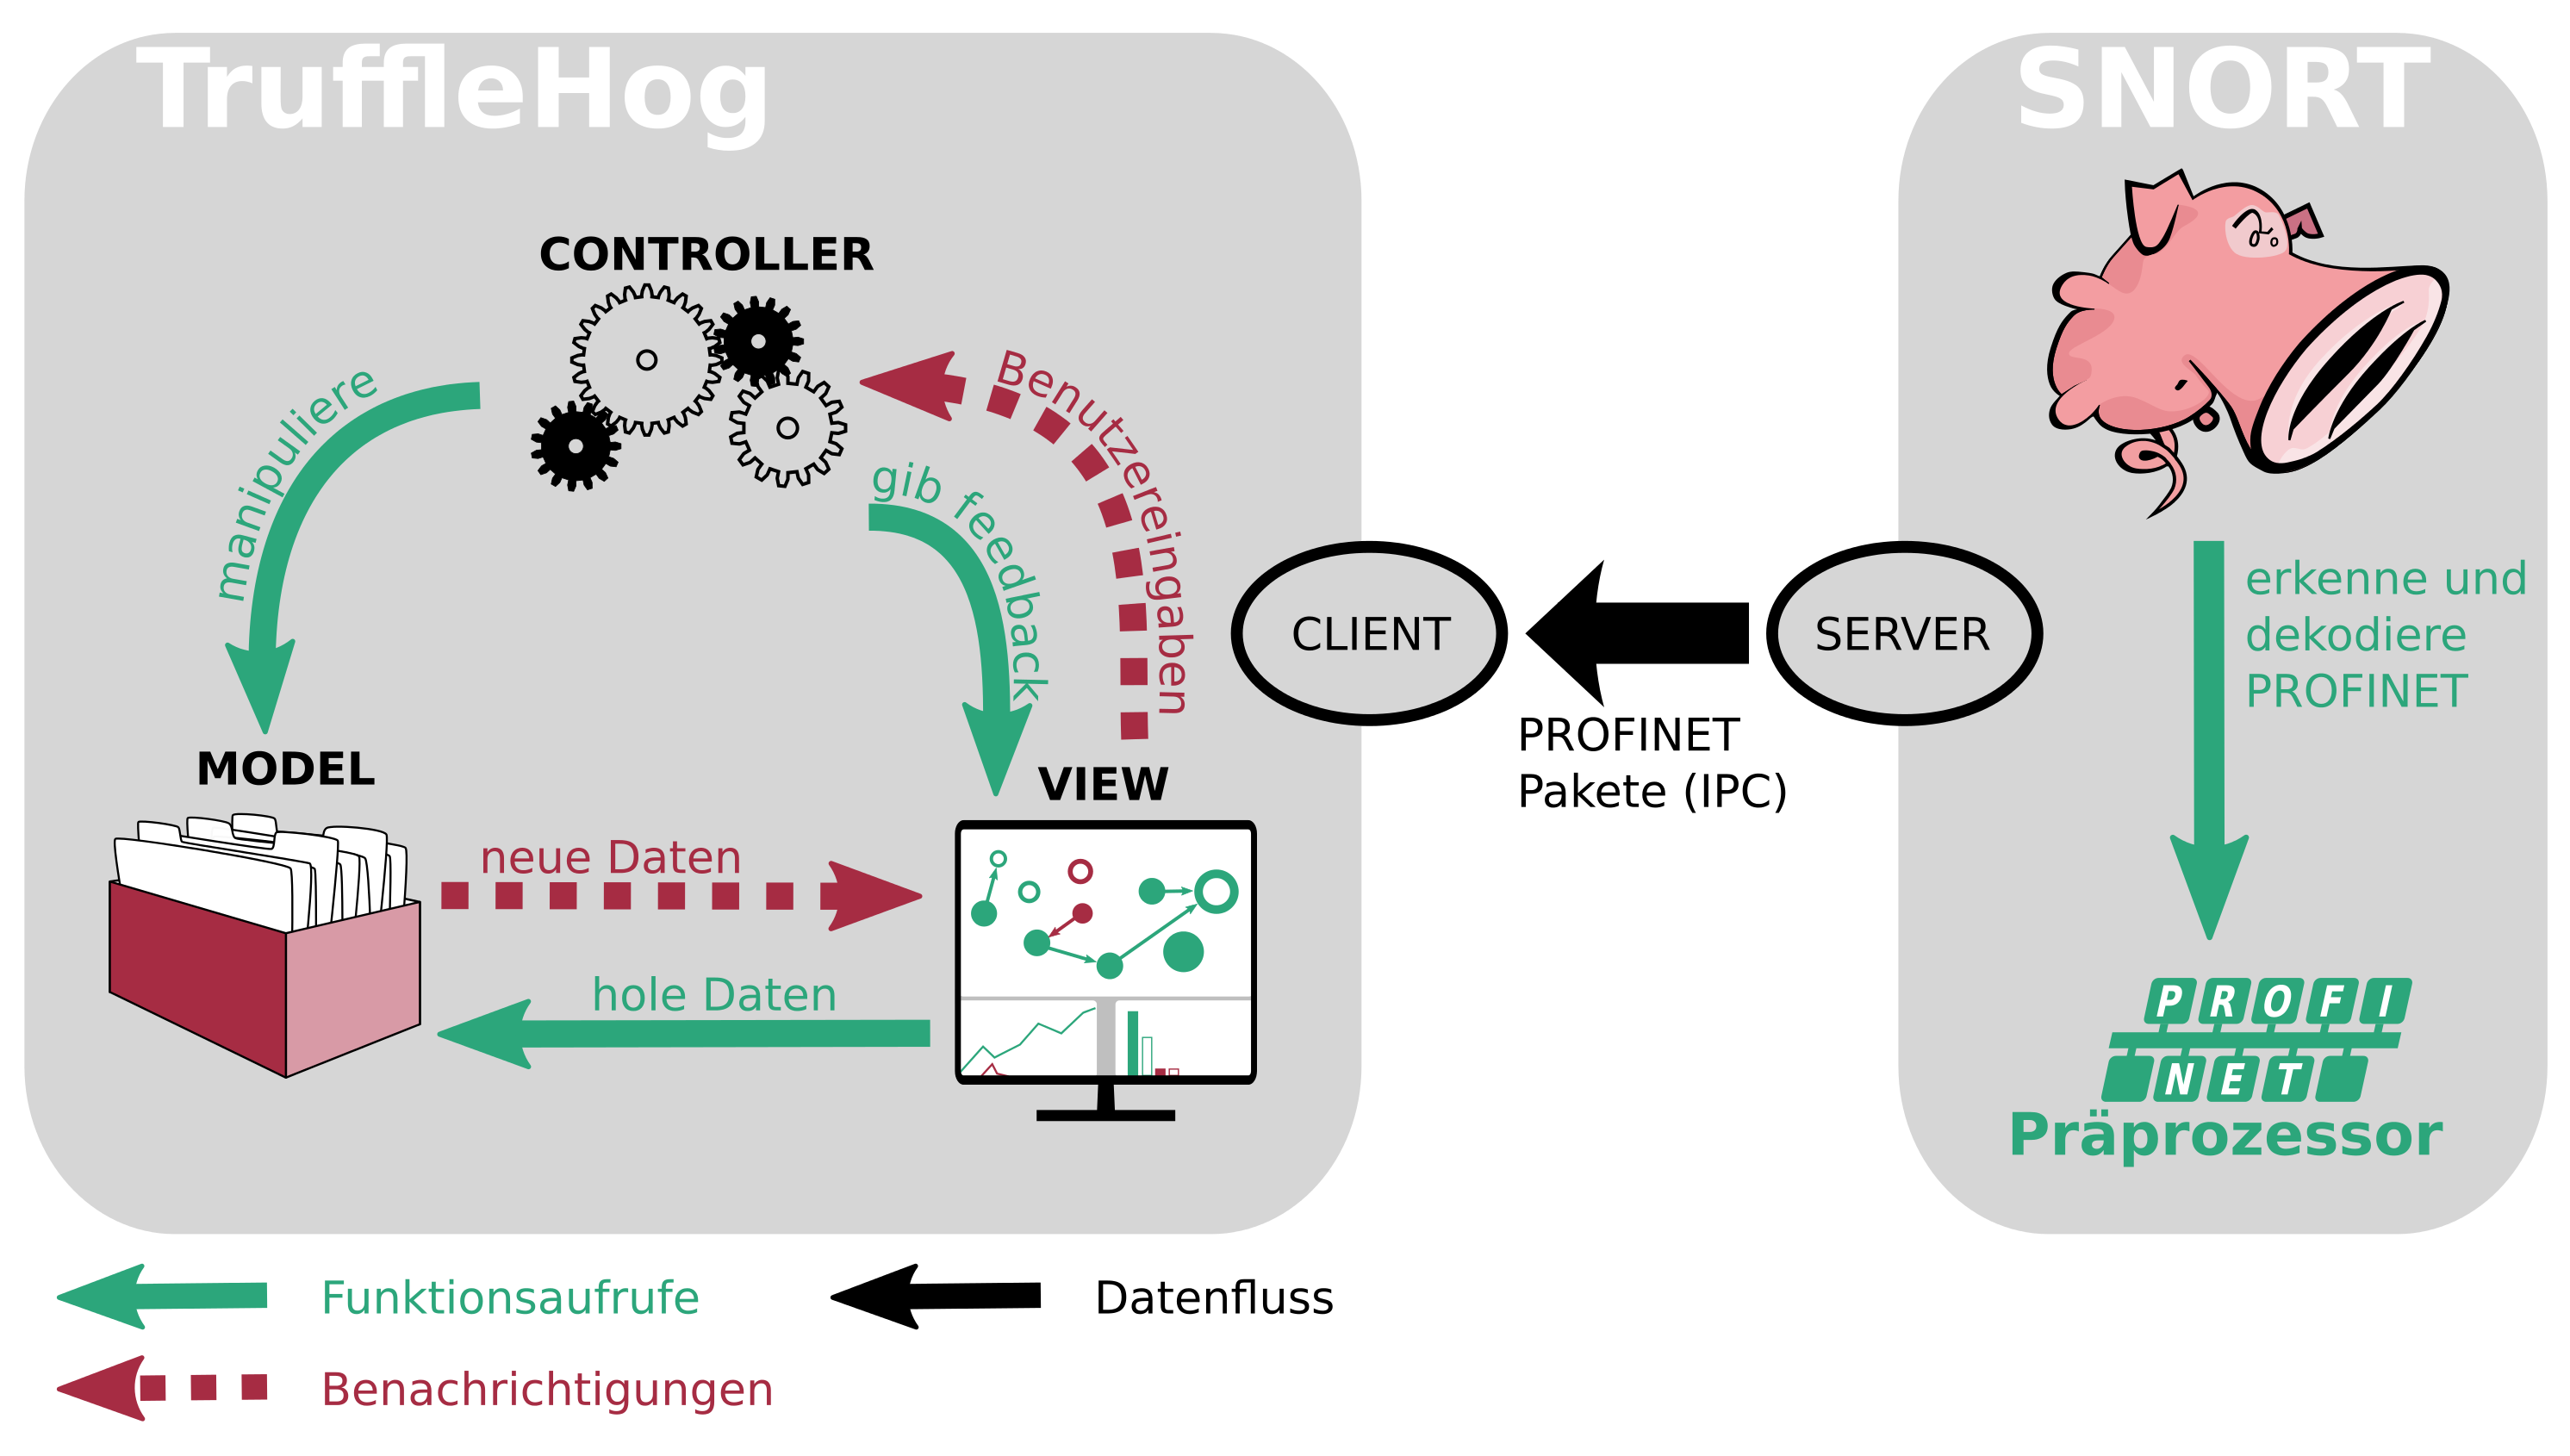
\includegraphics[width=0.8\textwidth]{../diagramimages/praesentationsmodel.png}
  \caption[Urspr''ungliche Architektur''ubersicht]{Urspr''ungliche Architektur''ubersicht}
  \medskip
  Ursprünglicher Aufbau der Programme aus dem Pflichtenheft
\end{figure} 

\begin{figure}[H]
  \centering
  \includegraphics[width=0.8\textwidth]{../diagramimages/arch_diagram_mvp_single.pdf}
  \caption[Erweiterte Architekturu''bersicht]{Erweiterte Architekturu''bersicht}
  \medskip
  Erweiterte Strukturierung des Programms nach dem \gls{mvp}
\end{figure} 

\chapter{Aufbau}

\section{\sppname}
\chapter{Aufbau \sppname}

\section{Architekturbeschreibung}

Sinn und Zweck dieses \gls{snort} \gls{praeprozessor}s \sppname ist das Abfangen, Komprimieren und Weiterleiten speziell von \gls{profinet}-\glspl{paket}n. Diese sind am \gls{ethertype} erkennbar, er muss der Hexadezimalzahl 0x8892 entsprechen. Des Weiteren soll der \gls{praeprozessor} über eine Reihe von erweiterbaren Decodern wichtige Informationen aus dem empfangenen \gls{paket} auslesen und in eine von uns vordefinierte Datenstruktur names Truffle schreiben. Pro Netzwerk-\gls{paket} entsteht also ein Truffle. Dieses wird dann per \gls{ipc} an unser \programname //valentin: ich mach hier weiter//
\section{Paketbeschreibung}


\section{\programname}
\subsection{Architekturbeschreibung}
Im Groben gehalten funktioniert der Daten- und Befehlsfluss im Trufflehog-Entwurf
wie im klassischen MVC, der Presenter aktiviert Services, welche das Model basierend
auf dem empfangenen Netzwerkverkehr verändert und das View aktualisiert sich am Model.
Da viele Threads im Programm parallel durchlaufen aber dennoch kommunizieren müssen,
verlassen wir uns an einigen Stellen auf das \gls{observerpattern} mit einer
Multi-Thread kompatiblen Datenstruktur.\newline
\newline

\subsection{Paketbeschreibung}

\subsubsection{command}

Die Kernfunktionalität innerhalb des Programms stellt das \textbf{command Paket}.
Darin befinden sich sowohl die Hierarchie, vorhandene Datenstruktur als auch jede
mögliche Command-Klasse und deren Interface. Vom Prinzip her vergleichbar mit
Runnables.\newline

\begin{figure}[H]
  \centering
  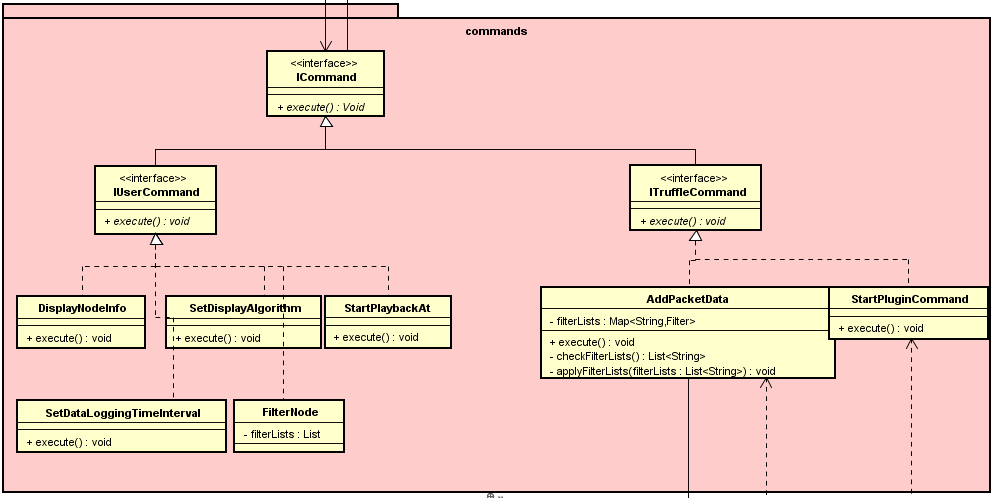
\includegraphics[width=\textwidth]{../diagramimages/commands.png}
  \caption{command Paket}
\end{figure}

Es gibt 2 Hauptarten von Commands, UserCommands für die Verwaltung der
Benutzeroberflächenbefehle, und TruffleCommands für die Methodenaufrufe im
Model-Graph, also die Hauptarbeit am Model. Die Commands machen außerdem den
Hauptteil der Log-Datein und damit der Video-Funktion aus. Mehr dazu im
service-Unterpackage datalogging.

\paragraph{Command Queue}
Die besagte Datenstruktur, welche beispielsweise der executor besitzt. Es
sind ggf. mehrere tatsächliche Queues vorhanden, was einen Manager verlangt
um nach dem Round-Robin-Prinzip faire Verteilung zu ermöglichen.


\subsubsection{service}


In unserem Entwurf haben wir uns außerdem dazu entschieden einzelne
durchlaufende Arbeitsschritte in das service Paket auszulagern.\newline

\begin{figure}[H]
  \centering
  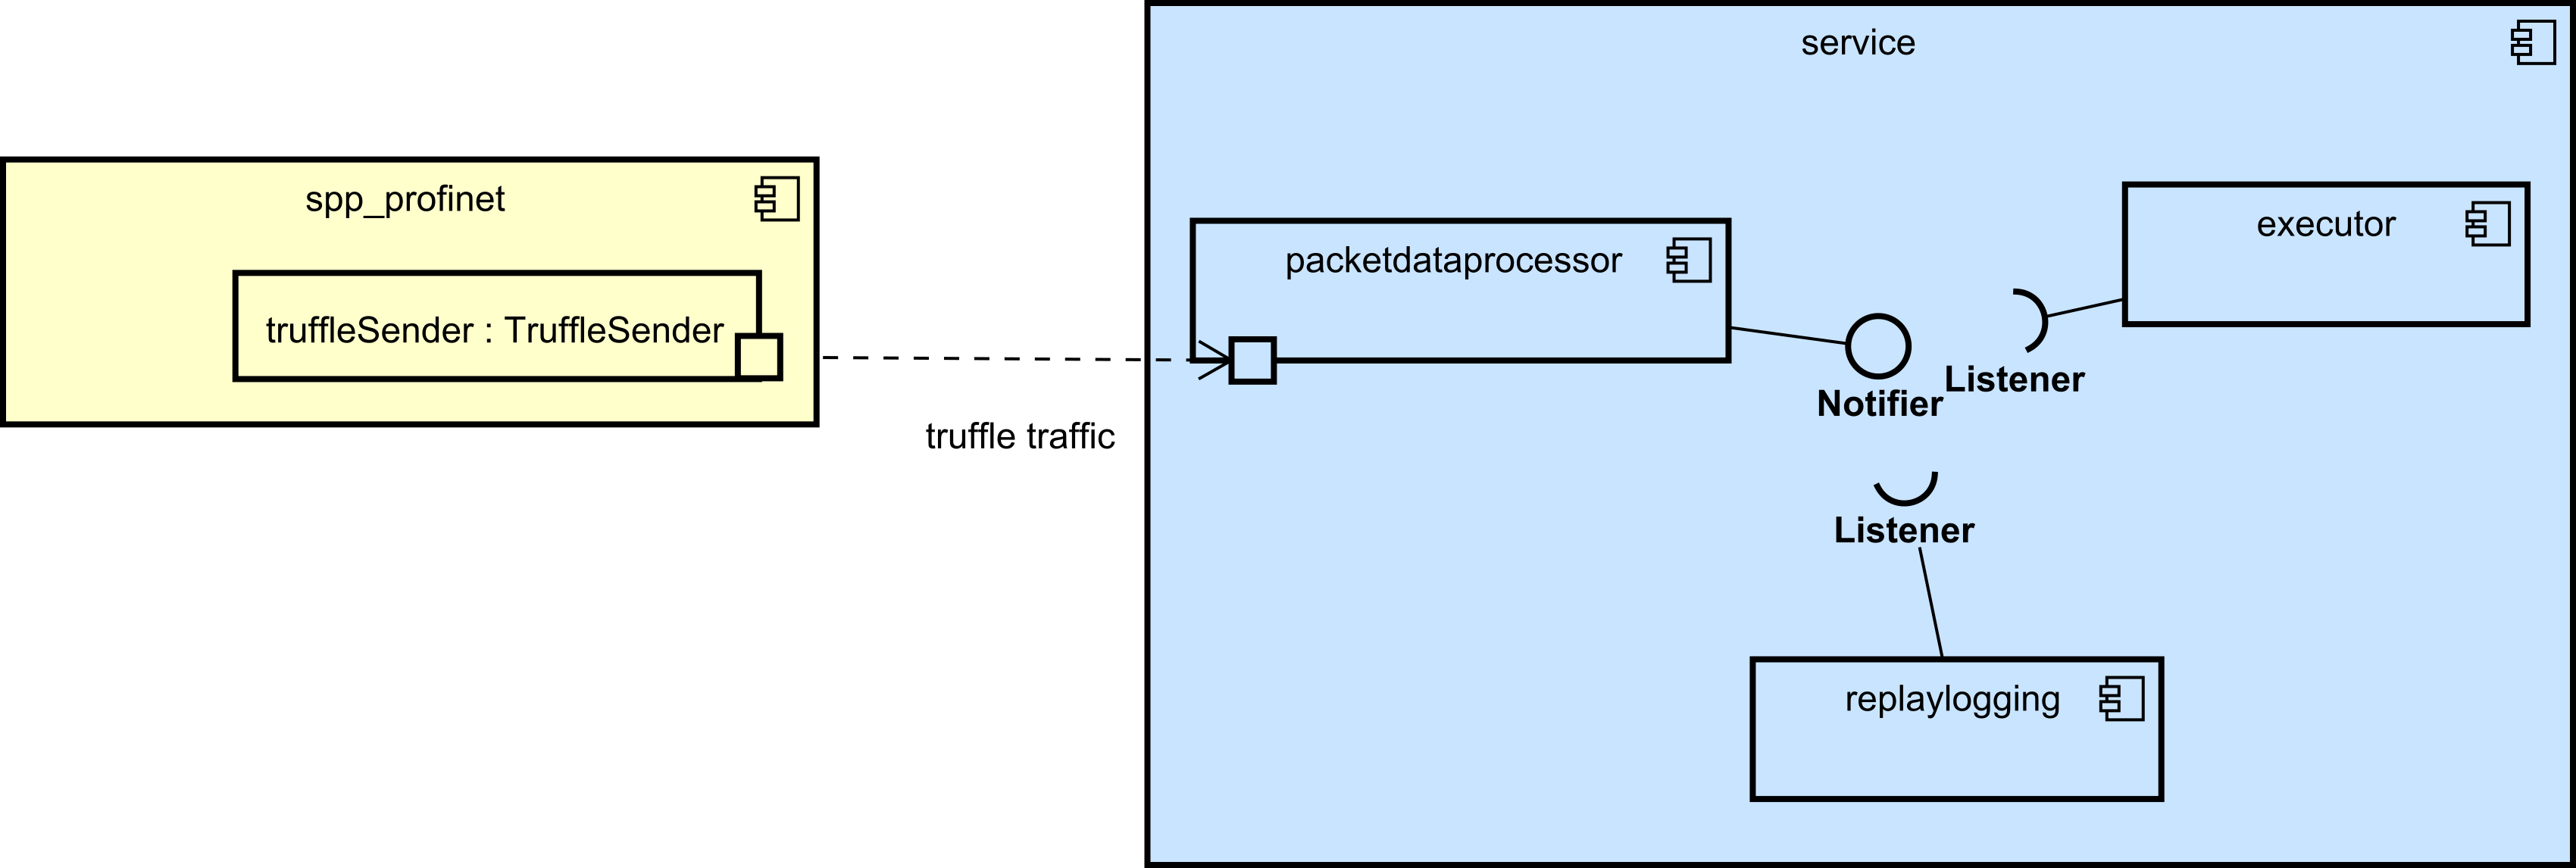
\includegraphics[width=\textwidth]{../diagramimages/service.png}
  \caption{service Paket}
  \medskip
\end{figure}

    \paragraph{truffleprocessor}
    Der truffleprocessor ist die Empfangsstelle für die von uns in der
    \gls{ipc} benutzen Truffles. Außerdem erzeugt er die später verwendeten
    Commands und benachrichtigt als \gls{notifier}.

    \paragraph{datalogging}
    Das datalogging kümmert sich um die gesamte gewünschte
    Speicherung/Loggen und, falls implementiert, die Verfügbarkeit der
    Video-Daten. Es speichert sowohl regelmäßige Snapshots des gesamten
    Graphen, als auch einzelne Commands für eine Schrittweise Rückverfolgung
    des Ablaufes.

    \paragraph{executor}
    Der executor ist das Unterpackage, in welchem die Anwendung bzw.
    Ausführung der Commands stattfindet. Er ist ein \gls{listener} für Commands
    von sowohl dem view-Package als auch dem truffleprocessor.


\subsubsection{presenter}


Der presenter ist für den Aufbau von \gls{programname}, also das
Initialisieren, Instanziieren und Referenzieren aller Programmelemente zuständig.

\begin{figure}[H]
  \centering
  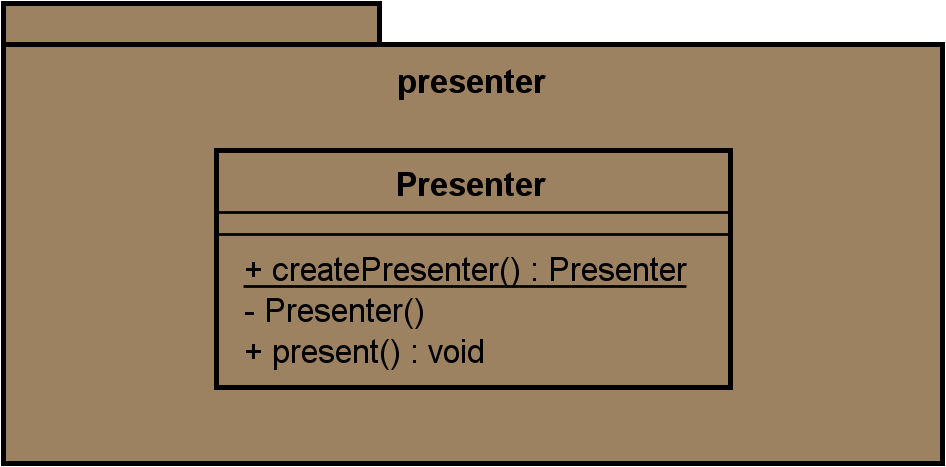
\includegraphics[width=\textwidth]{../diagramimages/presenter.png}
  \caption{presenter Paket}
\end{figure}

Er ist der erste Thread und erzeugt alle weiteren, zum Beispiel einen für jeden
Service. Außerdem liest er aus einer Settings-Datei und stellt das Programm ein.
Das heisst er initialisiert bestimmte Attribute entsprechend. Danach erschöpft
sich die Nützlichkeit des presenter bis zu einem neuen Programmstart.


\subsubsection{util}


Unsere Variante des \gls{observerpattern}s.

\begin{figure}[H]
  \centering
  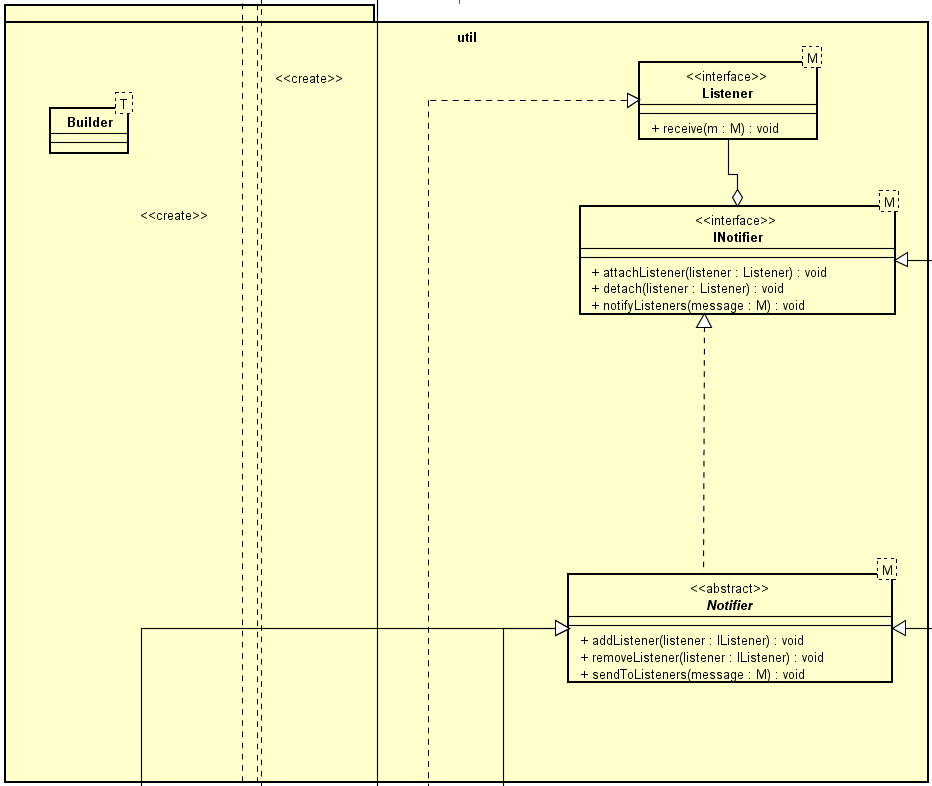
\includegraphics[width=\textwidth]{../diagramimages/util.png}
  \caption{util Paket}
\end{figure}

Da wir sowohl Interfaces als auch Klassen bzw. abstrakte Klassen als
\gls{notifier} haben, kommen wir nicht um eine Modifizierung des klassischen
\gls{observerpattern} herum. Nun haben wir die Möglichkeit sowohl ein
\gls{notifier}-Interface zu erweitern als auch eine abstrakte
\gls{notifier}-Klasse zu beerben. Der \gls{listener} funktioniert genau wie ein
Observer.


\subsubsection{model}


Die Hauptdatenstruktur von \gls{programname}: das model Paket.

\begin{figure}[H]
  \centering
  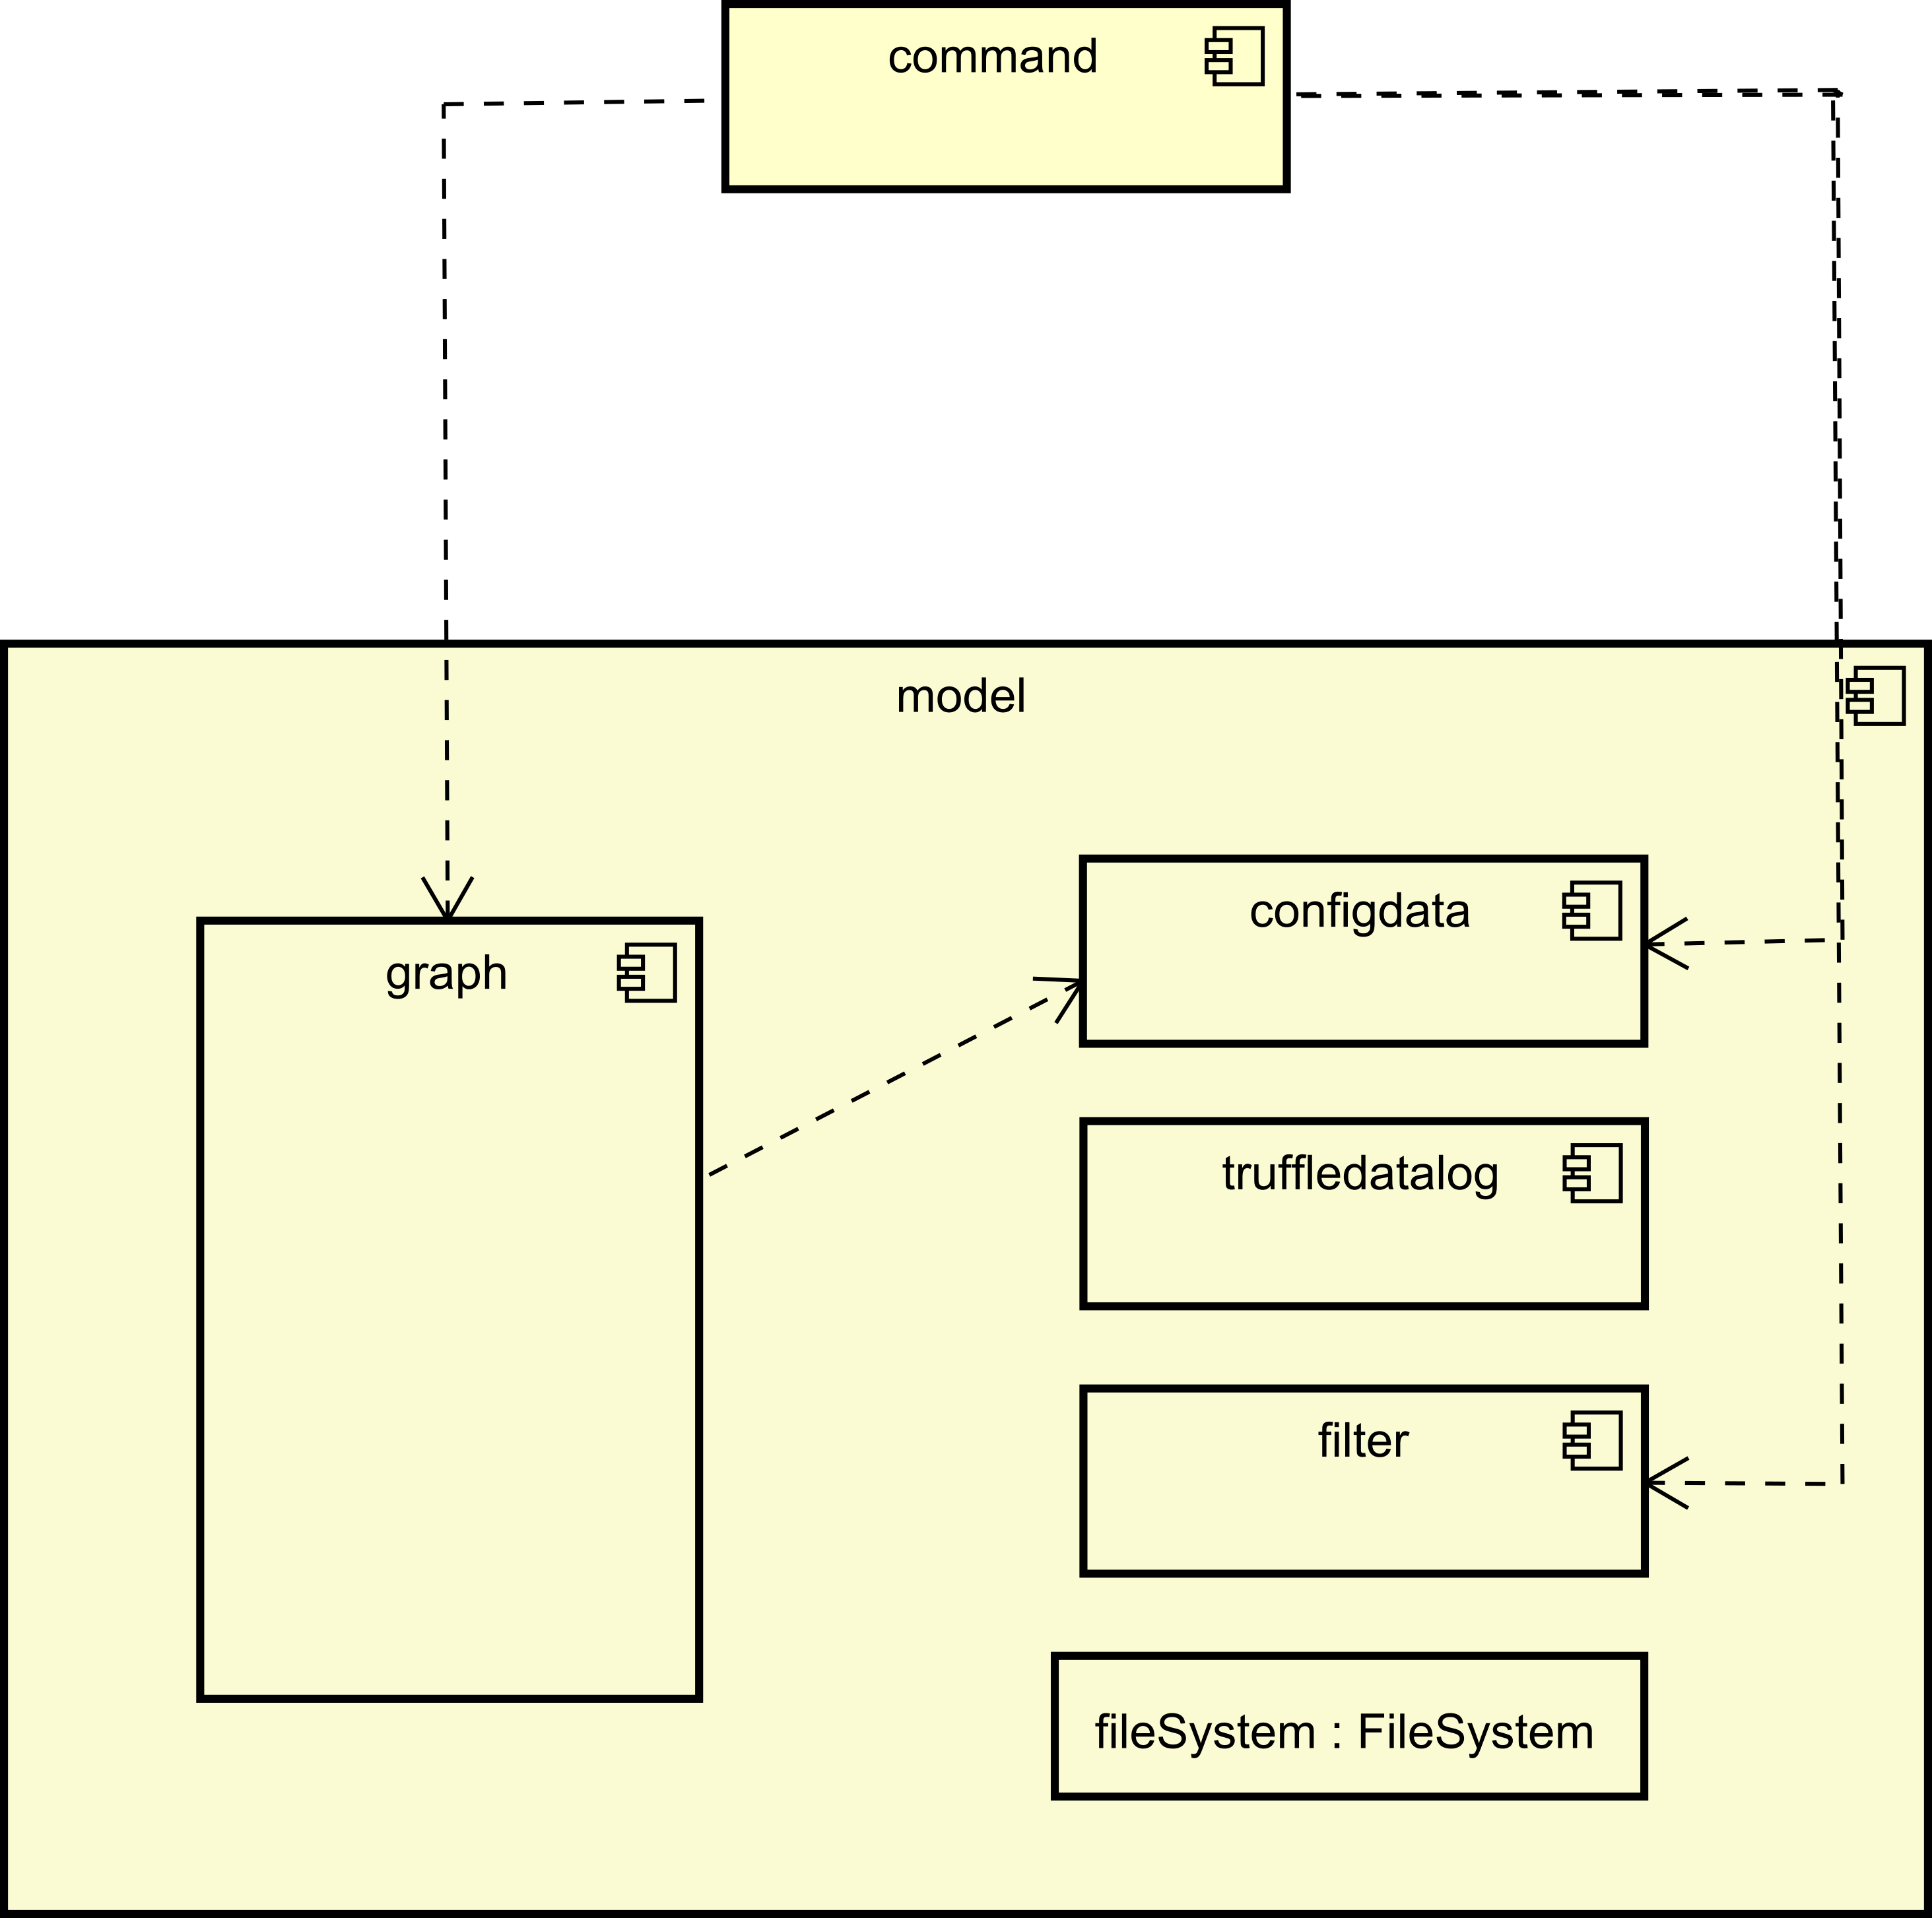
\includegraphics[width=\textwidth]{../diagramimages/model.png}
  \caption{model Paket}
\end{figure}

    \paragraph{graph}

    \paragraph{filter}

    \paragraph{settingsdata}

    \paragraph{graphlog}


\subsubsection{view}


\subsubsection{interactors}



\chapter{Abläufe}

\section{Präprozessor}

In dieser Sequenz werden zwei zentrale Aufrufe von \gls{snort} im \gls{praeprozessor} \gls{sppname} dargestellt. Zum einen im oberen Teil die Initialisierung des \gls{praeprozessor}s durch einen Init-Aufruf, sowie der \gls{praeprozessor}-interne Aufbau des DissectorRegisters. Dieser Registrierungsvorgang wurde im Diagramm aus Platzgründen eingespart. Darin wird jeder als C-Datei vorhandene Dissector instanziiert und bei dem DissectorRegister: TopLevelRegister registriert. Dieser Vorgang legt die Grundlage für den Dissector-Baum-Ablauf, welcher exemplarisch als zweiter unterer Teil des Sequenzdiagramms modelliert wurde. Für jedes empfangene Paket ruft \gls{snort} die detectProfinetPackets-Methode in \gls{sppname} auf und übergibt eine Paketpointer. Basierend auf dem Ethertype wählt der TopLevelRegister den ersten Dissector, den für ProfiNet-RealTimes (0x8892 Ethertype) aus und übergibt den Paketpointer. \gls{sppname} ruft in diesem Dissector die dissect-Methode auf, welche basierend auf gefundenen Informationen, sich einen passenden seiner Subdissector, hier den RT1Dissector, aussucht und in diesem die dissect-Methode aufruft. Dieser rekursive Schritt wird solange wiederholt, bis kein Subdissector mehr vorhanden ist oder das Ende des \gls{paket}s gefunden wurde.
Nach der Rückkehr der Methoden wird der fertige ProtocolTree benutzt und ausgelesen, um ein neues \gls{truffle} zu erstellen. Dieses selbstdefinierte \gls{truffle} wird dann mit dem Sender-Interface in Richtung \gls{programname} per \gls{ipc} verschickt.

\begin{figure}[H]
  \centering
  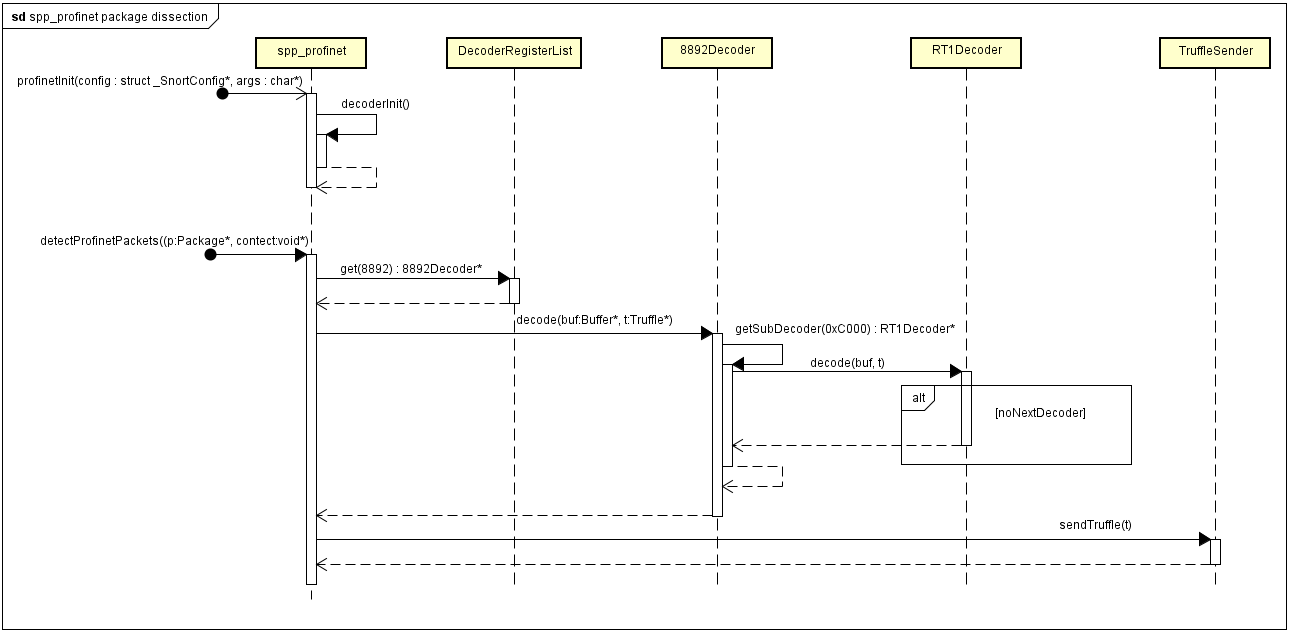
\includegraphics[width=\textwidth]{../diagramimages/spp-profinet-package-dissection.png}
  \caption[Sequenzdiagramm \gls{sppname} package dissection]{Sequenzdiagramm \gls{sppname} package dissection}
  \label{fig:spp_sqd}
\end{figure} 


\section{\gls{programname}}
\subsection{Receiver Executor communication}

Dieses Sequenzdiagramm beschreibt am Beispiel des CommandExecutors und des TruffleReceivers, wie das Notification Framework funktioniert.
Beide Services laufen in verschiedenen Threads. Der CommandExecutor nimmt solange Commands von seinen Queues, bis keine abzuarbeitenden
Commands mehr vorhanden sind. Falls dieser Fall eintreten sollte, so wird der thread schlafen gelegt, bis ein neues Element auf eine
der Queues geschrieben wird. Parallel dazu empfängt der TruffleReceiver von Snort Paketdaten und packt diese in Truffle. Anschließend
wird ein AddPacketDataCommand erstellt und das Truffle übergeben. Der Command wird dann mittels der receive Methode des CommandExecutor listeners
an diesen übergeben. Die receive Methode schreibt dann intern auf die CommandQueue des CommandExecutors. Dadurch wird dieser wieder aufgeweckt,
um die neuen Commands abzuarbeiten.

\begin{figure}[H]
  \centering
  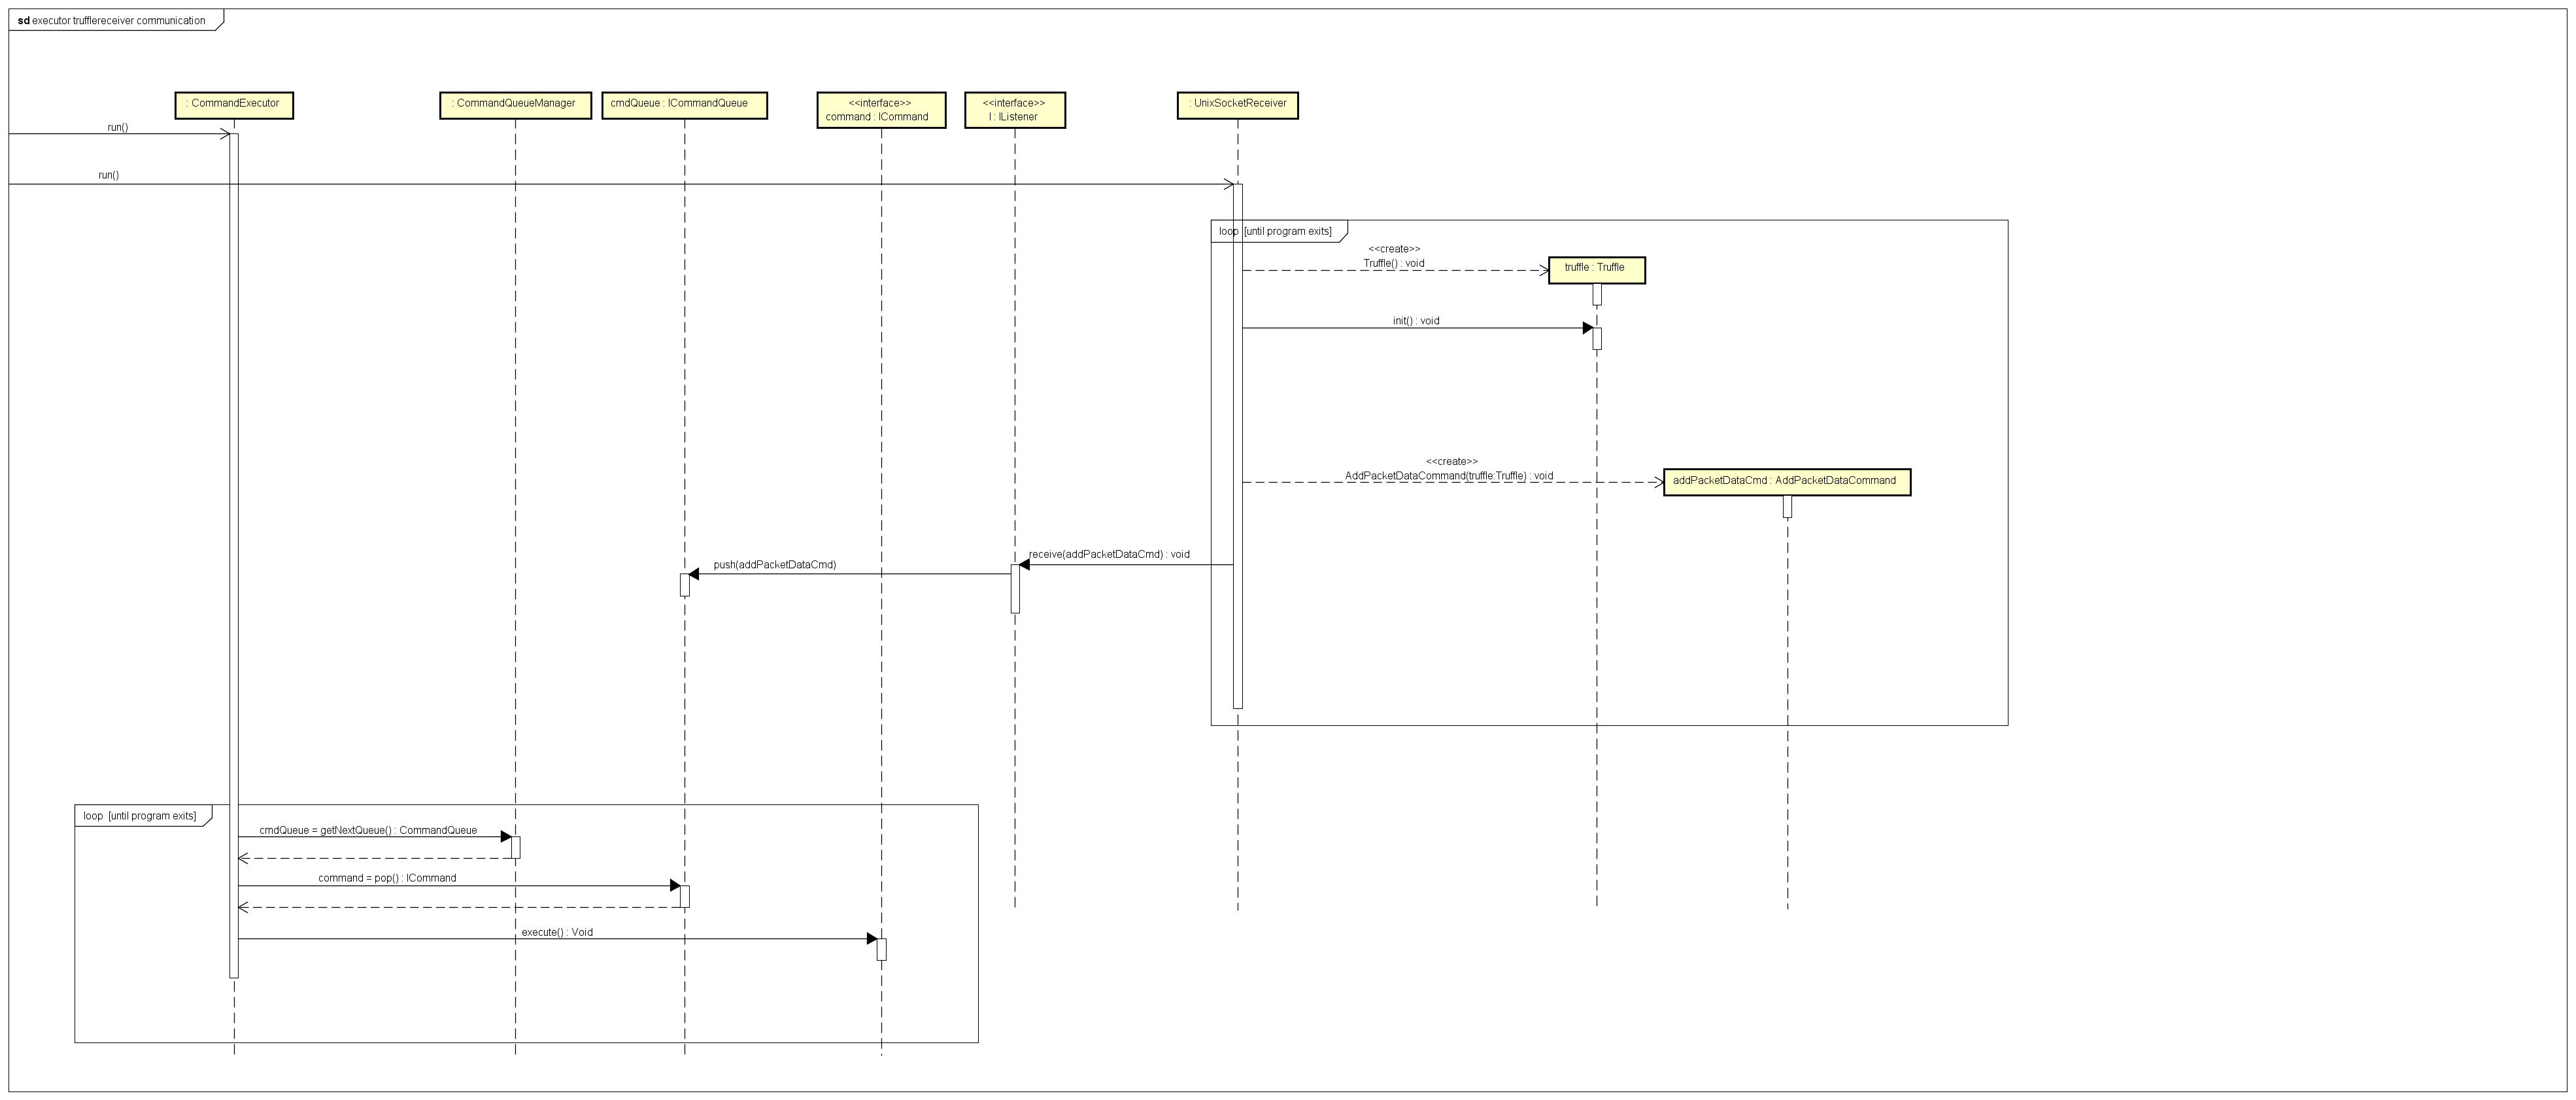
\includegraphics[width=\textwidth]{../diagramimages/sd_receiver_executor_comm.png}
  \caption[Sequenzdiagramm Receiver Executor communication]{Sequenzdiagramm Receiver Executor communication}
\end{figure}
\subsection{AddPacketDataCommand}
\begin{figure}[H]
  \centering
  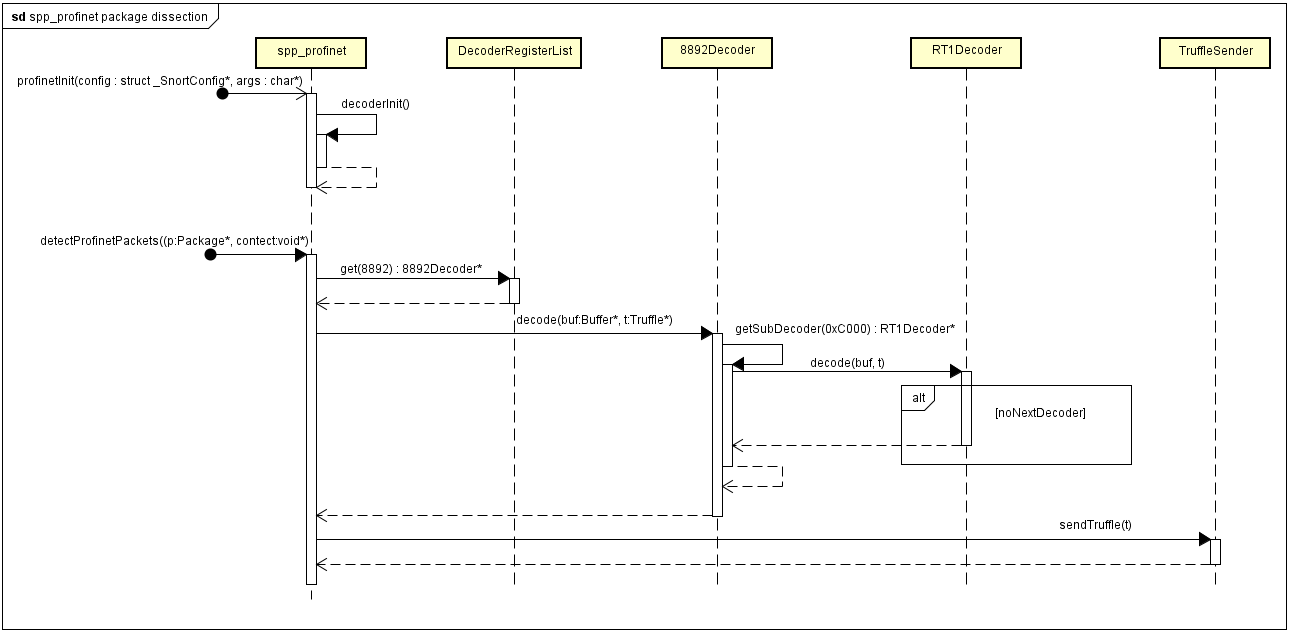
\includegraphics[width=\textwidth]{../diagramimages/spp-profinet-package-dissection.png}
  \caption[Sequenzdiagramm AddPacketData]{Sequenzdiagramm AddPacketData}
\end{figure}

Lorem ipsum dolor sit amet, consetetur sadipscing elitr, sed diam nonumy eirmod tempor invidunt ut labore et dolore magna aliquyam erat, sed diam voluptua. At vero eos et accusam et justo duo dolores et ea rebum. Stet clita kasd gubergren, no sea takimata sanctus est Lorem ipsum dolor sit amet. Lorem ipsum dolor sit amet, consetetur sadipscing elitr, sed diam nonumy eirmod tempor invidunt ut labore et dolore magna aliquyam erat, sed diam voluptua. At vero eos et accusam et justo duo dolores et ea rebum. Stet clita kasd gubergren, no sea takimata sanctus est Lorem ipsum dolor sit amet.
\subsection{DIAGRAMM}
\begin{figure}[H]
  \centering
  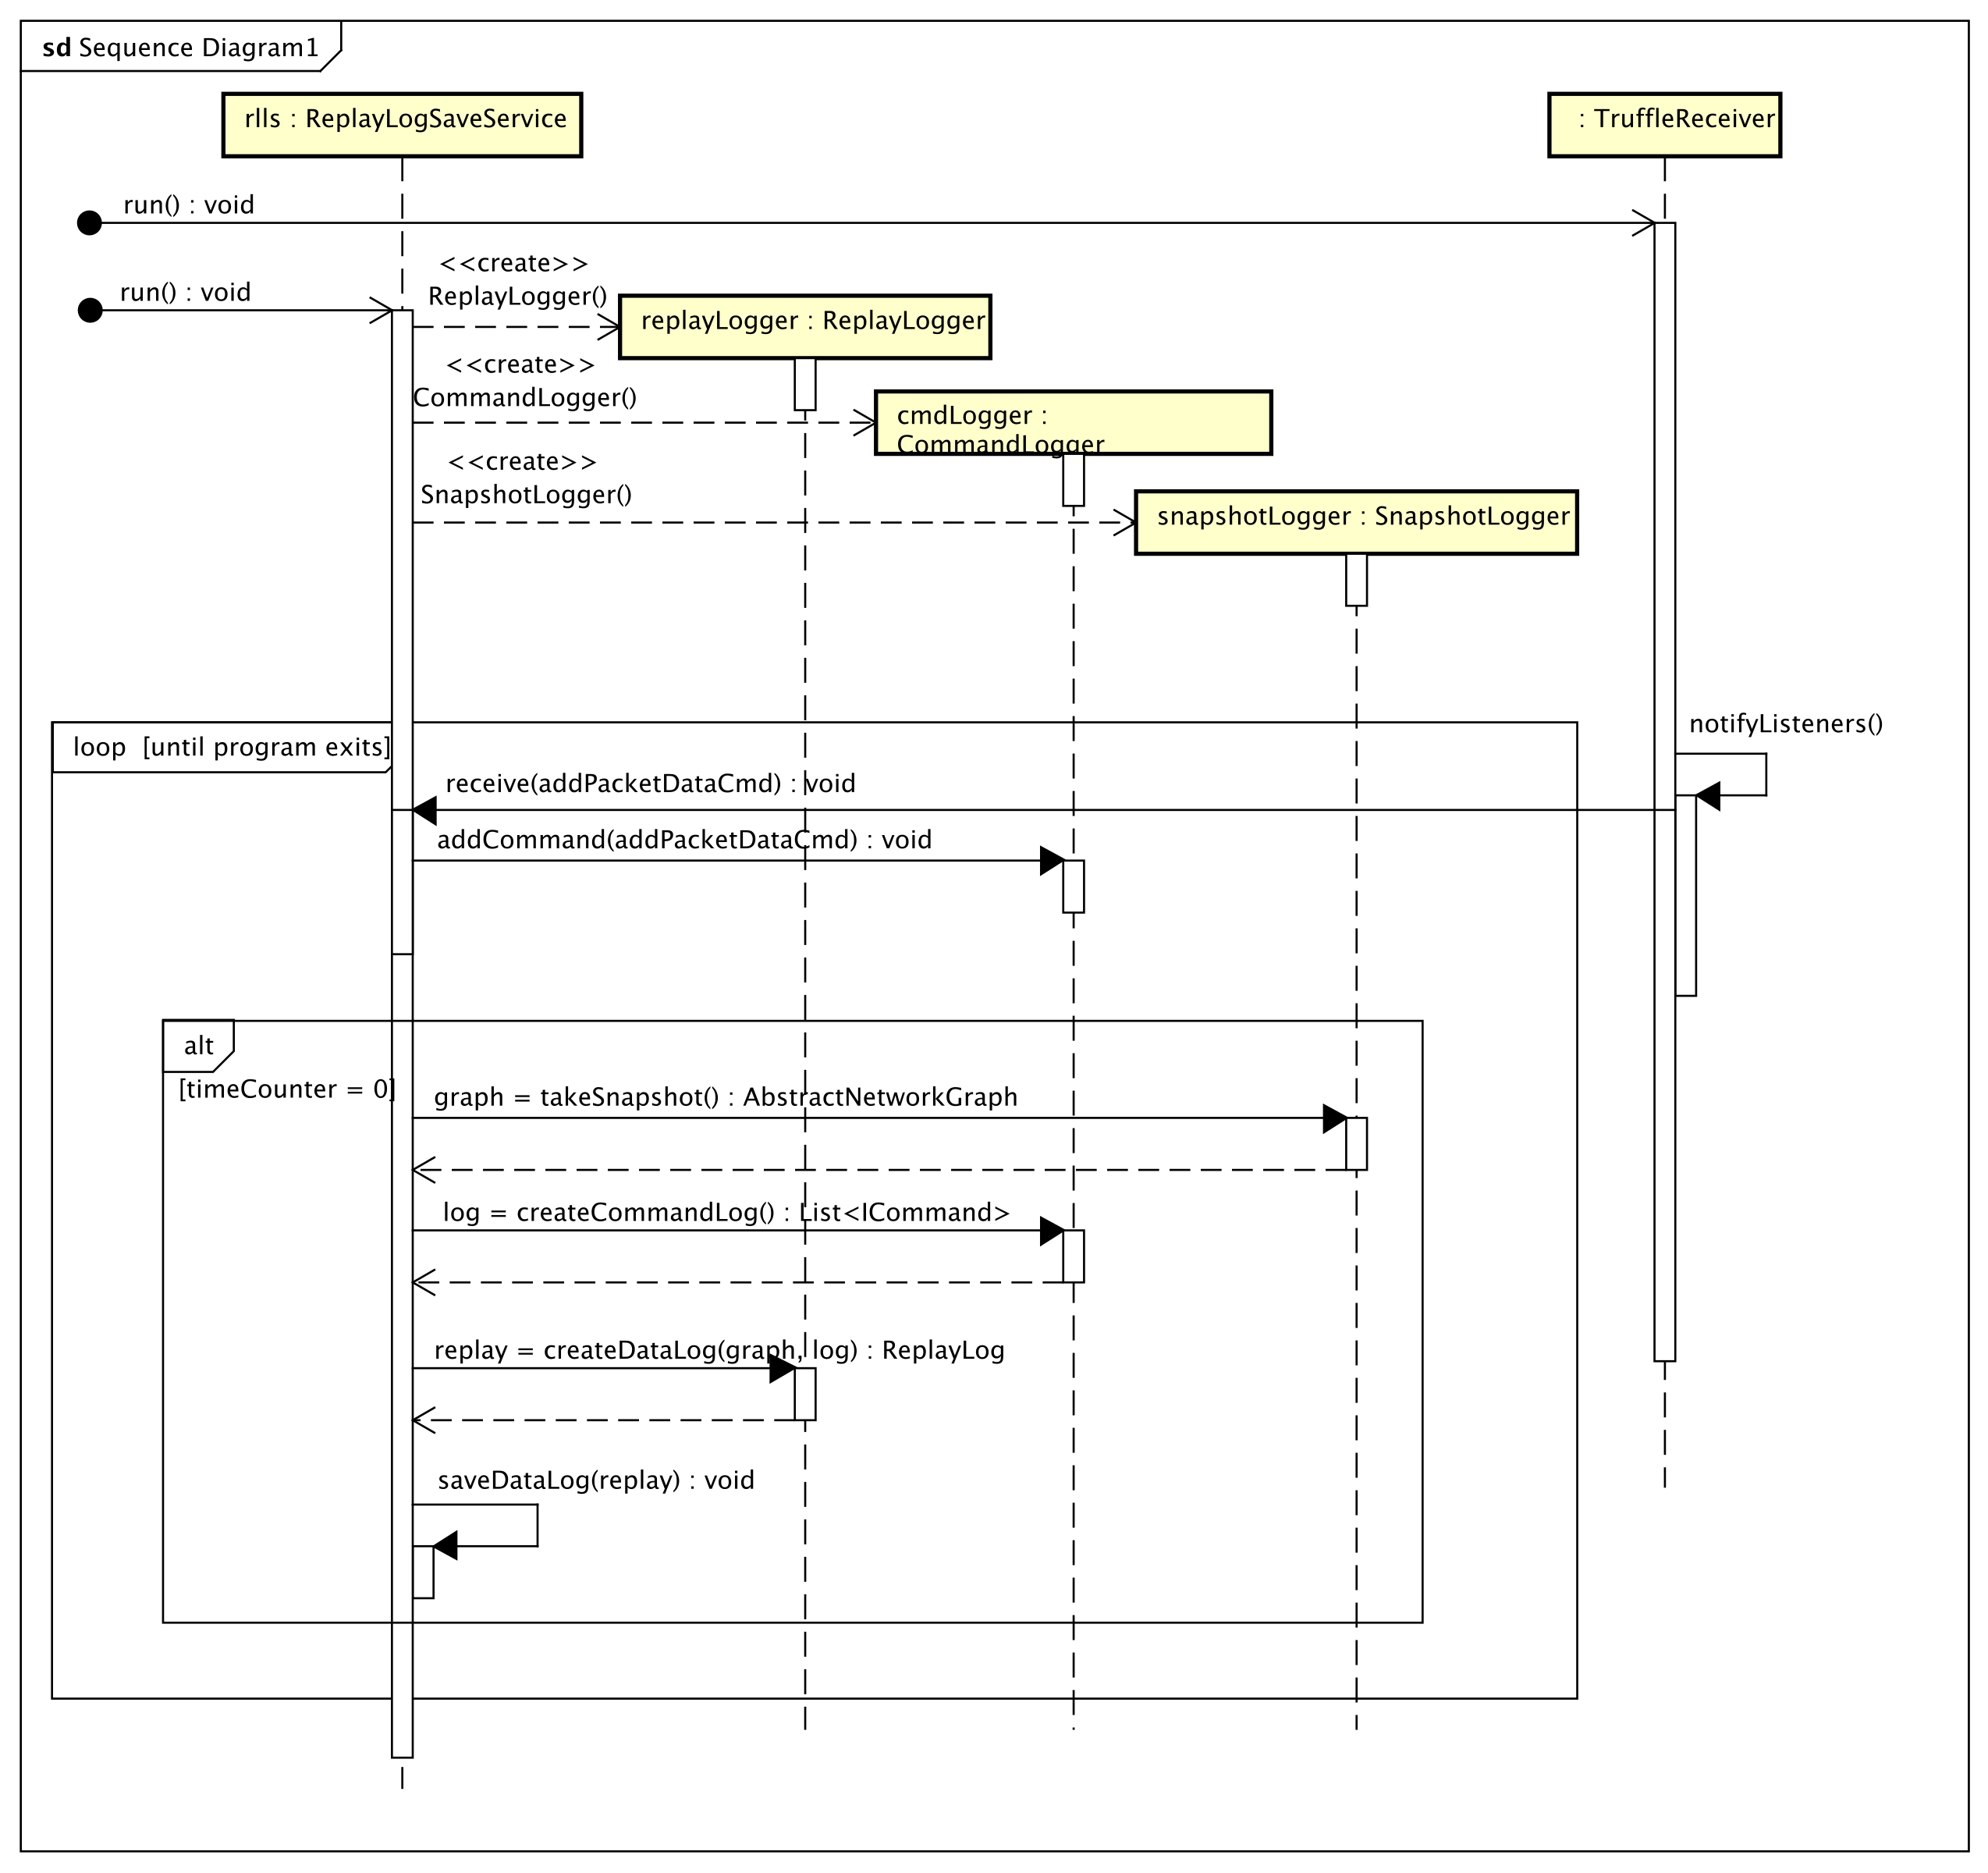
\includegraphics[width=\textwidth]{../diagramimages/sd_createsnapshot.png}
  \caption[Sequenzdiagramm DIAGRAMM]{Sequenzdiagramm DIAGRAMM}
\end{figure}

In diesem Diagramm wird die Ausführung des LoadSnapshotCommand dargestellt. Der Command wird von der View erstellt, falls der Benutzer versucht Replays anzusehen. Der Command ruft load() in dem ReplayLogLoadService auf. Dieser nimmt das übergebene Instant an und deserialisiert damit den ReplayLog. Dieser liefert den Graphen und die Commands. Im Proxy, der für den Replaygraph zuständig ist, wird der geladene Graph referenziert. Danach wird im ReplayLogLoadService das play-Flag gesetzt (da Service im eigenen Thread läuft, was zwecks besserer Übersicht ausgelassen wurde) und im NetworkGraphSwitch wird der aktuell dargestellte Graphen auf den Replaygraph umgestellt.
\subsection{DIAGRAMM}
\begin{figure}[H]
  \centering
  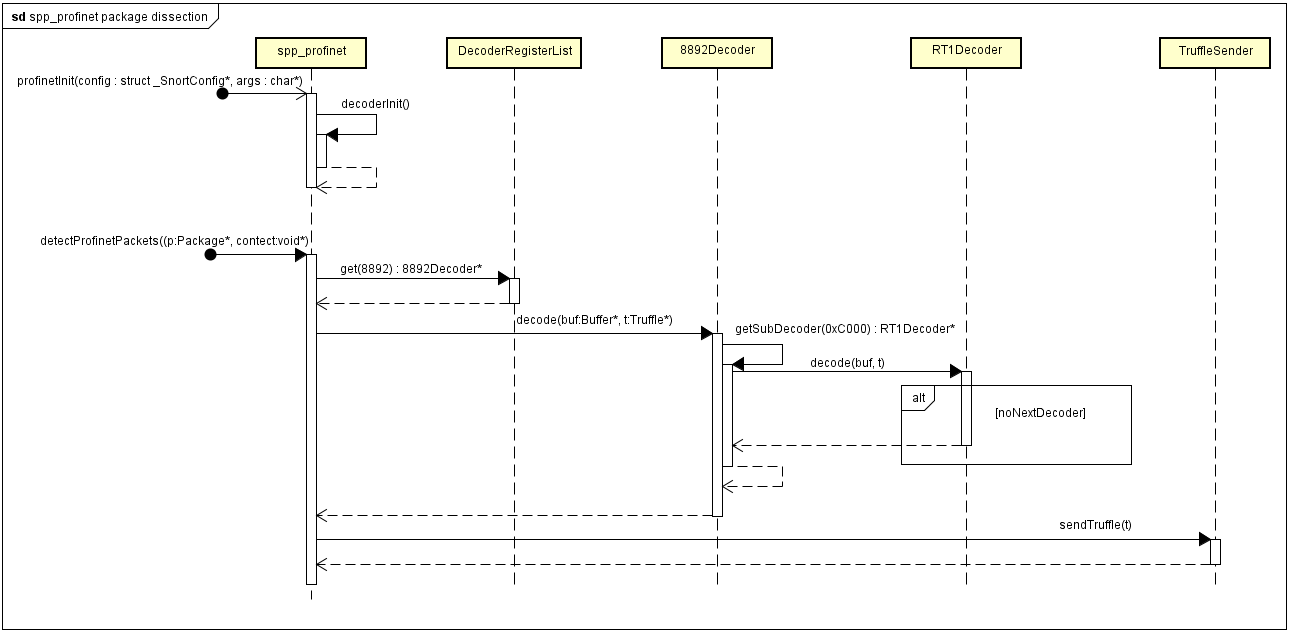
\includegraphics[width=\textwidth]{../diagramimages/spp-profinet-package-dissection.png}
  \caption[Sequenzdiagramm DIAGRAMM]{Sequenzdiagramm DIAGRAMM}
\end{figure}

 Das obige Diagramm zeigt die Speicherroutine der Commands und Snapshots des Graphen. Beim Start des ReplayLogSaveService erstellt sich dieser einen Replay-, Command- und Snapshotlogger, um sich später einen ReplayLog zusammenzustellen. Der ReplayLogSaveService ist ein Listener beim TruffleReceiver. Dadurch können die eingehenden Commands im CommandLogger gespeichert werden. Jeweils nach einem bestimmten Zeitintervall in der Endlosschleife wird ein Snapshot von dem Graphen erstellt und zusammen mit den gesammelten Commands in einem ReplayLog serialisiert. 

\chapter{Ressourcen}
\section{Dateien und Strukturen}
Im Folgenden ist das Datenhaltungsverzeichnis von \gls{programname} visualisiert. Alle persistenten, das heißt einen Neustart des Programms überdauernden Daten sind in Dateien in Unterordnern des Ordners \texttt{data} gespeichert.  
\begin{figure}[htb]
  \centering
\begin{verbatim}
.
`-- data
    |-- config
    |   |-- filtermenu_en.properties
    |   |-- graphwindow_en.properties
    |   |-- logwindow_en.properties
    |   |-- notificationview_en.properties
    |   |-- settingsmenu_en.properties
    |   `-- statistics_en.properties
    |-- log
    |   `-- trufflehog.log
    |-- replay_log
    |   |-- graph_TIMESTAMP2.trufflesnapshot
    |   `-- graph_TIMESTAMP.trufflesnapshot
    `-- truffle_data_log
        |-- nodeA.xml
        `-- nodeB.xml
\end{verbatim}
  \caption[Ordner- und Dateiestruktur von \gls{programname}]{Ordner- und Dateiestruktur von \gls{programname}}
\end{figure}
\begin{itemize}
\item[\texttt{config}] Einen Neustart des Programms überdauernde Informationen über die visuellen Teile des Programms und Speicherung sprachlicher Lokalisierungen. 
\item[\texttt{log}] Zentrale Logdatei des Programms. 
\item[\texttt{replay\_log}] Gesamtzustand des Graphen zu einem Zeitpunkt plus Veränderungen über eine gewisse Zeitspanne. 
\item[\texttt{truffle\_data\_log}] Logdatei zu jedem Knoten mit zeilenweiser Auflistung der verarbeiteten Truffles.
\end{itemize}

\section{Externe Bibliotheken}
\subsection{Java Universal Network/Graph Framework}
Die Bibliothek Java Universal Network/Graph Framework (JUNG) ist eine seit 2003 entwickelte Java-Bibliothek zur Speicherung, Visualisierung und zu Rechnen mit Graphen und graphähnlichen Strukturen. Sie ist modular aufgebaut und kapselt alle oben genannten Funktionen in verschiedenen Bibliotheksteilen. Außerdem bietet sie erweiterte Funktionalitäten wie verschiedene Anordnungsalgorithmen, diverse Annotationsmöglichkeiten der Visualisierung und Algorithmen zur Graphanalyse. 
\subsubsection{Motivation}
JUNG hat alle für \gls{programname} relevanten Funktionen einer Graphbibliothek und bietet zudem folgende Vorteile gegenüber vergleichbaren Bibliotheken. 

Für sämtliche Klassen der Bibliothek werden Interfaces bereitgestellt. Dies bedeutet, dass ohne Kompatibilitätsverlust neue Funktionen eingebunden werden können. 

Die kritischen Komponenten, also die Visualisierung, Datenhaltung und Graphlogik ist in JUNG modular voneinander abgegrenzt. Dies ermöglicht die perfekte Einbindung in das \gls{mvc}-Konzept von \gls{programname}. Viele andere Graphbibliotheken koppeln Datenhaltung und Visualisierung und würden somit keine klare Trennung des \gls{mvc} ermöglichen. 

JUNG ist als sehr stabile und verlässliche Bibliothek bekannt, die Wert auf Kompatibilität und weitgehende Fehlerfreiheit legt. 

Die Vorteile davon, dass JUNG eine Open Source-Projekt ist verstehen sich von selbst. 

\subsubsection{Verwendungsbeschreibung}




\appendix

\printglossary[title=Glossar,toctitle=Glossar]

\end{document}
